\documentclass[11pt]{article}

\usepackage[backend=bibtex]{biblatex}
\usepackage[utf8]{inputenc}
\usepackage{amsmath}
\usepackage{amssymb}
\usepackage{anysize}
\usepackage{graphicx}
\graphicspath{ {./images/} }
\usepackage{color}
\usepackage{xcolor}
\usepackage{algorithm2e}
\usepackage{pgfplots}
\usepackage{hyperref}
\usepackage{booktabs}
\bibliography{bibliography.bib}

\usepackage{tikz}
\usetikzlibrary{shapes,arrows}

\definecolor{mygreen}{rgb}{0,0.6,0}
\definecolor{mygray}{rgb}{0.5,0.5,0.5}
\definecolor{mypurple}{rgb}{0.58,0,0.82}

\usepackage{listings}

\usepackage{caption}
\DeclareCaptionFont{white}{\color{white}}
\DeclareCaptionFormat{listing}{\colorbox{gray}{\parbox[c]{\textwidth}{#1#2#3}}}

\setlength\parindent{0pt}
\setlength{\parskip}{10pt}

\marginsize{2cm}{2cm}{1cm}{1cm}

\usepackage{titlesec}
\titleformat{\section}{\large\bfseries}{\thesection}{1em}{}

\begin{document}

%  Title and authors
   \begin{center}
     {\huge\bfseries B31XP Robotics project\\ Robotic object follower}\\
      \vspace{2ex}
      \textsc{Andrey Pak, Donatas Kozlovskis, Enric Cornellà,\\ Fernando Garcia,  Igor Peric}
   \end{center}
   \vspace{2ex}%

%  Abstract
\begin{abstract}
This project presents a small, easy to build low-cost robot system, that is able to find coloured signs on the floor and implement the associated actions, e.g. stop, turn, pause, etc.
The robot hardware uses Raspberry Pi to control a set of motors, sensors and servo actuators. 
Report provides information about done review the hardware design and implementation of software using open source tools as C++ and OpenCV libraries. 
\end{abstract}

\section{Introduction}

Nowadays automation and robotics are leaving the traditional sectors as industrial manufacturing and becoming a part of daily life. It is integrating into our society, while many members still do not have a knowledge of it, since they are only familiar with the form of automation learned from massive social media.
Because of this trend of automation, it is important that educational organizations start preparing not only robotic researchers and designers, but also industrial personnel, who will be able
to take care of the robotic devices existing in our daily environment. 

A broad variety of robotic courses offered by universities or by massive open online education systems, increased during the past several years. However young students still lack opportunities to get hands-on experience on the understanding working principles, fabrication and implementation of robotic devices, which leads to the gap between theoretical and practical domain knowledge.

This project covered developing a low-cost wheeled robot, which is intended to promoting the teaching of basic computer science in schools \footnote{\url{http://www.raspberrypi.org/picademy/}}. Initial hardware design was provided by project supervisor, with limitations of only having motor servos, distance sensor, LCD screen, camera and Raspberry Pi (RPi) single-board computer.
Constraint of  Raspberry Pi computation power raised challenge to find an  optimal techniques of implementing controllers of sensors and actuators, knowing that the most of resources are consumed by image processing to implement and realise desired robot actions. Here, the optimal software design procedure is presented leading to the working example of constructed robot.


\section{Description of the Project}

\section{State of the art}

\section{Project Management}

In order to have a continuous progress, project management had to be established. The goal of management is to ensure that the whole project and software development process works as it is intended, allowing project activities to meet project requirements.
\\
The main steps of project management process are initiating, planning, executing, monitoring and controlling, and closing. Thus firstly, project team meetings were established on a weekly basis. Continuing defining the project goals, tight control of timeline had to be set as well, in order to keep track of deadlines.
\\
For this purpose the Gantt charts web tool\footnote{\url{https://teamgantt.com/}} was employed. It allowed to breakdown work structure of the project to small tasks, setting the start and finish dates individually. Example of Gantt chart used in this project can be seen in figure \ref{fig:gannt_example}.

\begin{figure}[ht!]
	\centering
	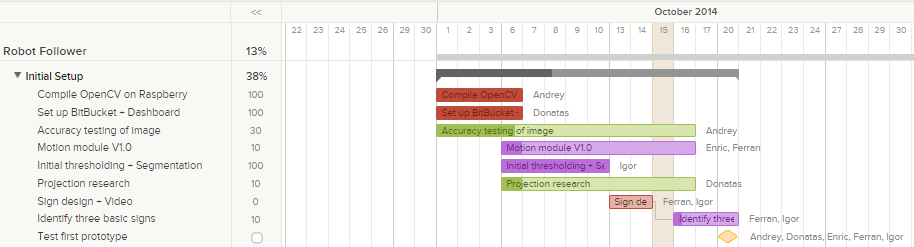
\includegraphics[width=1\textwidth]{gantt_chart_part}
	\caption{Part of planning represented on Gantt chart}
	\label{fig:gannt_example}
\end{figure}

Beside the track of the tasks, version control system for tracking the code changes had to be chosen. Common tools are Team Foundation Version Control, Mercurial or Git source control. Due to affordability and compatibility, distributed version control system Git was chosen. 
\\
For hosting the central GIT repository the two main players are \textit{Github} and \textit{Bitbucket}.
The main difference between the two is being cost for non-open source projects. \textit{Bitbucket} is free for teams up to 5 users and can host private closed source repositories whereas \textit{Github} does not provide private repositories for free. Thus the specifications of providers led to choose \textit{Bitbucket} for being web-based hosting service for this project.
\\
After setting up source version control, actual developing had started. In order to keep track with the Gantt chart, specific issues were created and assigned to each team member on a weekly basis. Project management tool \textit{Bitbucket Cards}, a part of \textit{Bitbucket}, offered interaction with issues on one easy-to-use, intuitive dashboard, where progress of tasks from one list to the next was easy to track.  Example of early stage project board can be seen in figure \ref{fig:bitcards}.

\begin{figure}[ht!]
	\centering
	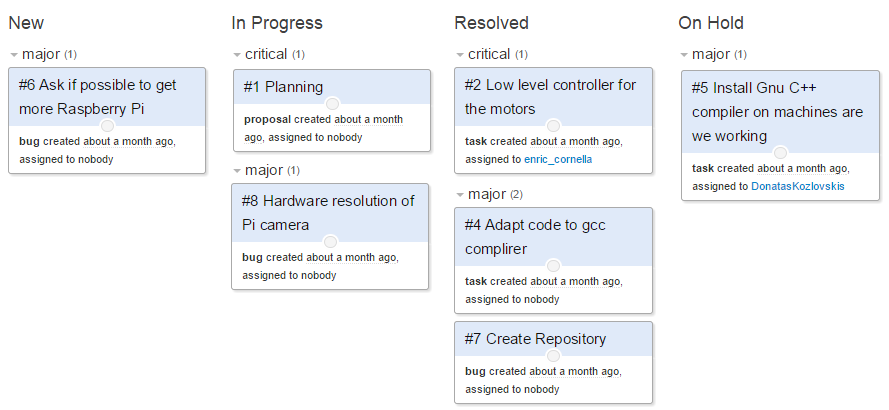
\includegraphics[width=0.7\textwidth]{bitbucket_cards}
	\caption{Early stage project board}
	\label{fig:bitcards}
\end{figure}

All mentioned tools were employed until the end of the project, resulting on continuous envelopment and progress.

\section{Implementation}
\clearpage
\subsection{Overview}
\subsection{Hardware}
\subsection{Software}
\subsubsection{Actuators and sensing drivers}
Most of the processes the robot is doing need either to get some information from external sensors or to send data to the actuators or displays. This is useful in the two ways of the communication. Sensors will give information to the robot so it can sense better the environment and act in consequence of what is happening in the \textit{exterior} world. Actuators, or output peripherals, give feedback to the persons interacting with the robot. A clear example would be explaining some instructions in an LCD screen or playing some sounds in certain actions of the robot. This will make the interaction easier and enrich the experience. Whenever it is needed to communicate with external devices, the robot needs to use drivers.

Next, the sound and LCD modules are explained as output devices and ultrasonic sensor and the push button as input device. It is important to remark that, although the motion module is run using drivers, it will not be explained in this section since a special part is dedicated to it due its importance.

A driver is non other than a small program that allows a computer (in the current case a Raspberry Pi) to communicate with some external devices. It gives basic instructions and functions to make an easy interaction between the both parts.

In this point it is important to remark two different groups of devices. The first one includes the sound module, which is already built in the Raspberry Pi making it easy to connect by simply plugging a speaker using a 3.5mm jack. It also includes the push button, wired directly to the GPIO. The second group, formed by the ultrasonic sensor and the LCD screen need an $I^{2}C$ protocol in order to communicate with the RPi.

For the first group it is needed an external speaker that can be easily plugged with a standard jack. In this case the Raspberry Pi already provides support for launching different sounds so it is straight forward to make it work. A button is also wired to the RPi in order to make an easy interaction when it is needed to start or stop the program without connecting the robot to a computer or external screen. 

The button is controlled by a \textit{Python} script that is initialized manually. When this program is running it will be constantly executed. Actually the program does nothing, it simply waits until a \textit{flag} is activated due to interaction with the button. It is connected to the GPIO of the RPi in \textit{normally open} mode, closing the circuit when it is pressed.

For giving an example of how this two parts work together, whenever the button of the robot is pressed a sound is played in order to give feedback to the children about the starting or shutting down of the program. The script receives a \textit{flag} that the button has been pushed and an instruction like \textit{os.system('omxplayer sound.mp3')} reproduces a sound. In figure \ref{fig:module1} it is possible to observe how the button and speaker are connected to the Raspberry Pi. The ports used for the button are the pin number 24 and any \textit{GND}.

\begin{figure}[h]
\centering
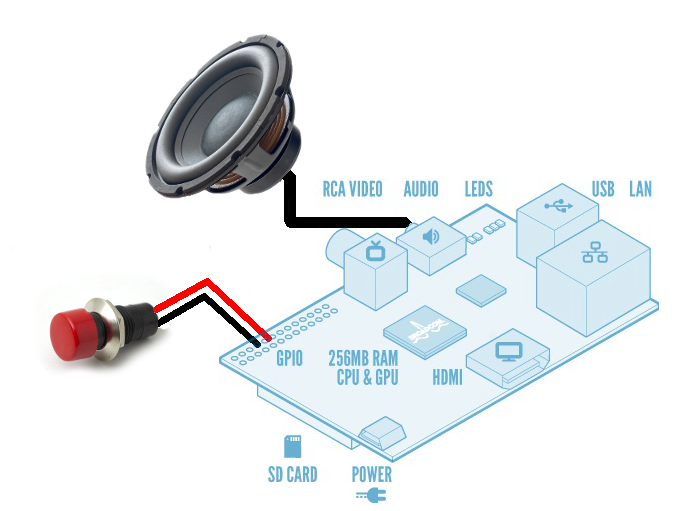
\includegraphics[width = 0.6\textwidth]{module1}
\caption{Connection of the external speaker and the button}
\label{fig:module1}
\end{figure}

In the second group a new protocol is introduced: $I^{2}C$, that refers to \textit{Inter Integrated Circuit}, a multi-master and multi-slave serial bus. It is a protocol used for attaching low-speed peripherals to embedded systems, small computers or microchips. The power of $I^{2}C$ is that allows to connect several devices in the same line of cables. By identifying each one of this devices with an unique address it is possible to control all of them. In figure \ref{fig:i2c} it is possible to observe the connection of the two devices that make use of $I^{2}C$. As can be seen only four cables are needed for sending and receiving data. Red and black are used as power source, typically +5V or +3.3V. Green and blue cables are Serial Data Line (SDA) and Serial Clock Line (SCL). The working principle of $I^{2}C$ is very simple. Each one of the devices has a specific address which is known a priori (certain addresses are available to chose for each device). When it is needed to communicate with one of them a buffer is sent to the correspondent address and the device acts in consequence. Later it is explained each one how it works.

\begin{figure}[h]
\centering
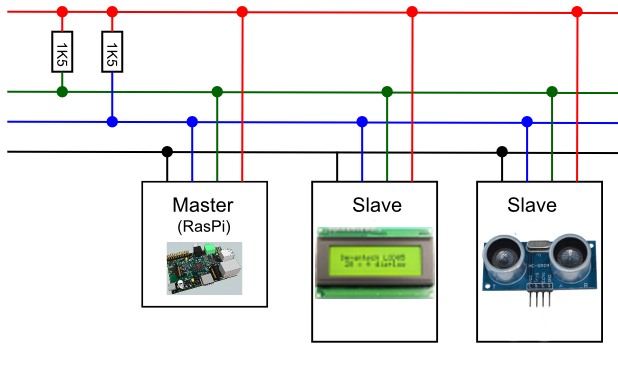
\includegraphics[width = 0.6\textwidth]{i2c}
\caption{Connection of multiple devices to a $I^{2}C$ port. Raspberry Pi is working as master while the other two peripherals are working as slave.}
\label{fig:i2c}
\end{figure}


The LCD display is used to show information about the current state of the robot. It is a very powerful way to know what the robot is thinking or doing without the need of connecting a screen to the Raspberry Pi. This is very important since the less computational power expended on the RPi the better. Avoiding the initialization of a graphical user interface will result in a slightly more fast execution of the program, which is desired. It is also a very nice way to communicate with children and explain maybe some instructions or the current state of the robot so they know what the robot is doing. The flow of the information in the $I^{2}C$ bus is only in one way, from the RPi to the LCD. Whenever it is needed to write something in the screen a command is sent via the bus and the device executes it. The two most common functions used are the ones to write and clean the screen.

The proximity sensor provides information to the robot about its surroundings. The working principle is based on ultrasonic sounds that rebound on objects. By calculating the amount of time for a sound wave to get back to the sensor it is possible to estimate the distance. In this case the $I^{2}C$ bus is working in two directions. In order to get data from the sensor first it is need to send some information to it. It is like a conversation where the RPi asks for information and the ultrasonic sensor responds with this data.In this way it is avoided to continuously receive unnecessary data. Grabbing distance two or three times per second is enough in the current case since the robot is not moving fast.

\subsubsection{Motion module}

This module had to realise control of robot wheels. Since designed robot uses
Dual 12Volt 2.8Amp H Bridge Motor Drive MD25 \footnote{\url{http://www.robot-electronics.co.uk/htm/md25i2c.htm}}, controlling the board is done using I2C bus system mode.
Generally this module had to realize following actions:
\begin{itemize}
	\item drive motors by setting individual speeds for both wheels;
	\item get heading of the robot by reading encoder values.
\end{itemize}
Thus these requirements led to splitting the whole module into two blocks:  one being responsible for driving motors and another for reading/writing encoders.

\begin{figure}[!ht]
	\centering
	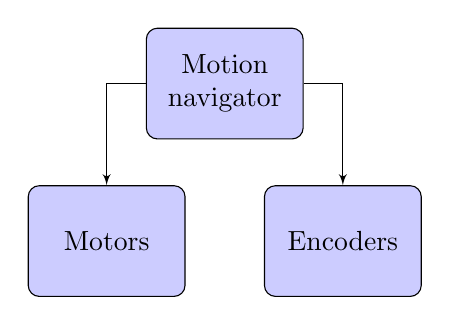
\begin{tikzpicture}[node distance = 2cm, auto]
	\tikzstyle{block} = [rectangle, draw, fill=blue!20, 
	text width=5em, text centered, rounded corners, minimum height=4em]
	\tikzstyle{line} = [draw, -latex']
	% Place nodes
	\node [block] (navigator) {Motion navigator};
	\node [block, below of=navigator, xshift=-1.5cm] (motors) {Motors};
	\node [block, below of=navigator, xshift= 1.5cm] (encoders) {Encoders};
	% Draw edges
	\path [line] (navigator) -| (motors);
	\path [line] (navigator) -| (encoders);
	\end{tikzpicture}
	\caption{Motion module structure}
	\label{fig:motion_structure}
\end{figure}

\subsection{Controlling motors}

All communication between high level functions and motors is done via  I2C bus command register.
The MD25 has 17 registers numbered 0 to 16 as follows:
\begin{table}[h]
	\begin{tabular}{@{}llll@{}}
		\toprule
		\textbf{Register} & \textbf{Name}     & \textbf{Read/Write} & \textbf{Description}                                             \\ \midrule
		0                 & Speed1            & R/W                 & Motor1 speed (mode 0,1) or speed (mode 2,3)                      \\
		1                 & Speed2/Turn       & R/W                 & Motor2 speed (mode 0,1) or turn (mode 2,3)                       \\
		2                 & Enc1a             & Read only           & Encoder 1 position, 1st byte (highest),   \\
		3                 & Enc1b             & Read only           & Encoder 1 position, 2nd byte                                     \\
		4                 & Enc1c             & Read only           & Encoder 1 position, 3rd byte                                     \\
		5                 & Enc1d             & Read only           & Encoder 1 position, 4th (lowest byte)                            \\
		6                 & Enc2a             & Read only           & Encoder 2 position, 1st  byte (highest),  \\
		7                 & Enc2b             & Read only           & Encoder 2 position, 2nd byte                                     \\
		8                 & Enc2c             & Read only           & Encoder 2 position, 3rd byte                                     \\
		9                 & Enc2d             & Read only           & Encoder 2 position, 4th byte (lowest byte)                       \\
		10                & Battery volts     & Read only           & The supply battery voltage                                       \\
		11                & Motor 1 current   & Read only           & The current through motor 1                                      \\
		12                & Motor 2 current   & Read only           & The current through motor 2                                      \\
		13                & Software Revision & Read only           & Software Revision Number                                         \\
		14                & Acceleration rate & R/W                 & Optional Acceleration register                                   \\
		15                & Mode              & R/W                 & Mode of operation (see below)                                    \\
		16                & Command           & Write only          & Used for reset of encoder counts and module address changes      \\ \bottomrule
	\end{tabular}
	\caption{The MD25 register}
\end{table}

For controlling the motors, registers 0, 1 and 15 are used. Firstly, when initializing motor control, mode register (15) is modified.
The mode register selects which mode of operation and I2C data input type the user requires. Here the type 3 was chosen and writing this value 
to the mode register makes enables turn mode: speed1 controls both motors \textit{speed}, and speed2 becomes the \textit{turn} value. 
Data is in the range of -128 for full reverse, 0 for stop and 127 for full forward speed of motors.

It is worth to mention, that turn mode looks at the speed register to decide if the direction is forward or reverse. Then it applies a subtraction or addition of the turn value on either motor. If the direction is forward
\begin{table}[!ht]
	\centering
	\begin{tabular}{lcl}
		motor speed1 & = & speed - turn;\\
		motor speed2 & = & speed + turn;
	\end{tabular}
\end{table}

else the direction is reverse 
\begin{table}[!ht]
	\centering
	\begin{tabular}{lcl}
		motor speed1 & = & speed + turn;\\
		motor speed2 & = & speed - turn.
	\end{tabular}
\end{table}

Manipulating mentioned registers, 4 main motor controlling functions were implemented as seen in figure \ref{fig:motor_structure}.
\begin{figure}[!ht]
	\centering
	\begin{tikzpicture}[node distance = 2cm, auto]
	\tikzstyle{block} = [rectangle, draw, fill=blue!20, 
	text width=5em, text centered, rounded corners, minimum height=4em]
	\tikzstyle{line} = [draw, -latex']
	% Place nodes
	\node [block] (motors) {Motors};
	\node [block, below of=navigator, xshift=-1.5cm] (stop) {Stop Motors};
	\node [block, left of=stop, node distance = 3 cm] (drive) {Drive Motors};
	\node [block, below of=navigator, xshift=1.5cm] (left) {Turn left};
	\node [block, right of=left,  node distance = 3 cm] (right) {Turn right};
	% Draw edges
	\path [line] (motors) -| (drive);
	\path [line] (motors) -| (stop);
	\path [line] (motors) -| (left);
	\path [line] (motors) -| (right);
	\end{tikzpicture}
	\caption{Motor controlling functions}
	\label{fig:motor_structure}
\end{figure}

\subsection{Controlling encoders}

For controlling the encoders, registers 2-9 and 16 are used.
Manipulating mentioned registers, 3 main encoder controlling functions were implemented, which are presented figure \ref{fig:encoder_structure}.
\begin{figure}[!ht]
	\centering
	\begin{tikzpicture}[node distance = 2cm, auto]
	\tikzstyle{block} = [rectangle, draw, fill=blue!20, 
	text width=5em, text centered, rounded corners, minimum height=4em]
	\tikzstyle{line} = [draw, -latex']
	% Place nodes
	\node [block] (encoders) {Encoders};
	\node [block, below of=navigator, xshift=-1.5cm] 	(rleft) {Read right encoder};
	\node [block, left of=stop, node distance = 3 cm] 	(lleft) {Read left encoder};
	\node [block, below of=navigator, xshift=1.5cm] 	(reset) {Reset both encoders};
	\node [block, right of=left,  node distance = 3 cm] (angle) {Get robot heading};
	% Draw edges
	\path [line] (encoders) -| (rleft);
	\path [line] (encoders) -| (lleft);
	\path [line] (encoders) -| (reset);
	\path [line] (encoders) -| (angle);
	\end{tikzpicture}
	\caption{Motor controlling functions}
	\label{fig:encoder_structure}
\end{figure}


\clearpage
\clearpage
\section{ Final setup }
\begin{itemize}
\item
Explain the final setup of the robot. Specially the things that were not included initially (IR camera, IR leds, button to start program).
\item
Testing results.
	\begin{itemize}
	\item
	How homography helps.
	\item
	How IR helps.
	\item
	How improvement of arrow angle detection helps.
	\end{itemize}
\item
Specifications achieved (fps, missdetections, etc.)
\end{itemize}

\section{Problems encountered}



\section{Further improvements}


\clearpage


\end{document}